\chapter{Mon stage}
\label{sec:unchapitre}

Lorsque j'ai répondu à l'offre de stage, il été avait initialement prévu que je produise une newsletter ainsi que trois vidéos sur trois APIs différentes qui sont :

\begin{itemize}
    \item Gat'Ape/Okapi
    \item Zbus
    \item Valkey
\end{itemize}

Cependant, aux vues de mon avancement et de l'intérêt suscité par les vidéos produites, j'ai accepté de travailler sur trois autres projets :

\begin{itemize}
    \item Explication des difficultés liées à la création et à la publication d'APIs avant l'arrivée du cloud au sein d'Orange
    \item Présentation des avantages du travail en DevOps
    \item Promotion de PnS.com
\end{itemize}

Les vidéos traitant des APIs se devaient d'être vulgarisées et simple à comprendre étant donné qu'elles pourraient être destinés à un public très vaste. Chaque vidéo se doit d'être compréhensible par un programmeur, un manager ou un commercial par exemple. La principale difficulté est de devoir vulgariser un maximum tout en gardant un maximum de précision pour qu'elles restent pertinentes pour les personnes les plus techniques. La diffusion de ces vidéos peut se faire pour montrer les dernières avancées au sein de la SDFY, ou encore pour promouvoir un produit, ou le proposer à des clients en tant que nouvelle solution. \\

En revanche, l'approche pour les 3 autres vidéos est totalement différente, elles s'adressent à un public ciblé et ont principalement un but promotionnel. Deux de ces vidéos ont été réalisées pour un événement particulier. \\

Avant de développer développer le contexte et la production de chaque vidéo, je vais d'abord présenter le programme PnS.com et ses différents composants. 

\section{Présentattion générale de l'écosystème PnS.com}

PnS.com est une extension de l'ancienne solution de stockage de données à haute performance et disponibilité appelé PnS. Cette extension le rend As A Service (AAS), c'est à dire accessible via internet par le client. L'architecture de PnS.com se divise en quatre parties.

\begin{itemize}
    \item Le backend
    \item Les injecteurs
    \item Le backoffice
    \item Les APIs
\end{itemize}

%%%%%%%%%%
% Schema %
%%%%%%%%%%

\begin{figure}[htp]
  \centering
  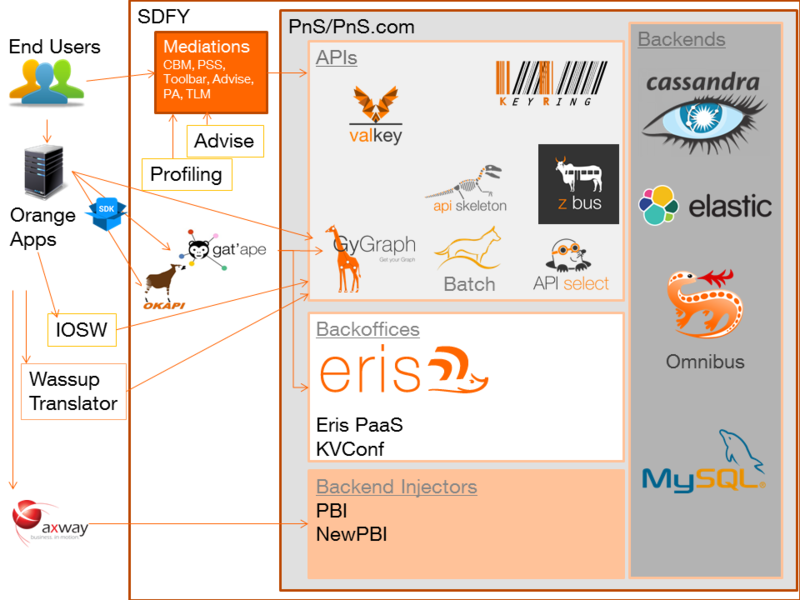
\includegraphics[width=15cm]{images/pns/psn.png}
  \caption{Schéma de l'architecture de PnS.com.}
  \label{pns}
\end{figure}


Le backend est composé de la base de donnée Cassandra noSQL, prévue pour stocker un grand nombre de données stockées sur plusieurs serveurs différents. Elle possède donc une haute disponibilité et possède un système d'élimination de ponts défaillants qui lui assure une quasi certitude d'accès aux données. Parmi le backend figure aussi Elastic Search qui est un moteur de recherche qui va faciliter la consultation de la base de donnée, et Omnibus sert de lien entre Cassandra et Elastic Search.\\

Les injecteurs quant à eux on le rôle d'envoyer en masse des informations dans la base de données.\\

Le backoffice, et plus particulièrement Eris, qui est l'outil de gestion des flux. Il permet à un service de type PnS de présenter l'ensemble de ses relations avec ses fournisseurs et ses partenaires. Ses principales fonctionnalités sont de pouvoir rechercher de l'information par mot clef, mais aussi de saisir de l'information et de pouvoir suivre les flux.\\

Enfin, les APIs sont présentes pour ajouter des fonctionnalités à l'écosystème PnS.com. Parmi ces APIs, nous retrouvons Batch, qui va permettre des injections, Select, qui va permettre de faire des recherches sous forme de texte comme nous le ferions dans un moteur de recherche au lieu d'utiliser les noms des variables. Skeleton, socle pour les APIs, Zbus, dont le but est de transmettre des messages \textit{(cf : 2.3)}, GyGraphe qui permet de modéliser une base de donnée sos forme de graphe et Valkey qui fournit le modèle clef/valeur \textit{(cf : 2.4)}.\\

Actuellement, 185 applications se connectent à PnS quotidiennement, ce qui représente 20 000 requêtes/s en lecture et 8 000 requêtes/s en lecture sur la base de données. Ces applications viennet de milieux différents tels que le portail orange.fr, encore l'espace client ou bien encore le Suivi Conso par exemple. Ces applications viennet chercher des données, que cela soit les leurs ou bien des données provenant de référentiels, ou bien une grande capacité de stockage et une scalabilité sans impact. En effet, PnS dispose de 70TB qui permettent d'absorber les variations de volume de stockage.

\section{Vidéo sur Gat'Ape/Okapi}

\subsection{Contexte}
Gat'ape/Okapi est une API faisant partie de l'écosystème PnS.com qui permet d'exposer, de s'authentifier et de sécuriser les APIs de cet écosystème. Gat'ape et Okapi ont deux fonctions bien distinctes.\\

Okapi est le système d'authentification qui va permettre la connexion aux autres APIs. Okapi est basé sur le couple Oauth2/Kerberos qui va permettre une identité indépendante à chaque entité tout en offrant un système d'authentification unique (SSO) qui va permettre à l'utilisateur d'accéder à plusieurs applications en ne s'authentifiant qu'une seule fois. Cette authentification repose sur un système de clé secrète et de jeton. Il est à noter que des options de sécurité plus complexes sont aussi disponibles.\\

Gat'ape quant à elle est la passerelle qui va permettre d'exposer les APIs, c'est à dire, des les rendre visible à d'autres utilisateurs pour qu'ils puissent s'y connecter. Gat'ape va pouvoir offrir un contrôle d'accès et un contrôle de trafic permettant de réguler le flux des utilisateurs. Gat'ape est également responsable  de l'authentification et de la sécurité lors de la consommation par Okapi. En plus de cela, gat'ape est également scalable, c'est à dire qu'elle va pouvoir maintenir son activité et sa performance même lors d'une forte demande.\\

Dans les faits la connexion grâce à Gat'ape/okapi se passe comme suit : 
L'application qui vient se connecter possède une clé secrète. Cette clé secrète est envoyée à Okapi. Lors du traitement, Okapi va renvoyer un jeton d'authentification unique au consommateur ainsi qu'un digest. Ceci est la phase d'authentification.  Ce digest est ensuite envoyé du consommateur vers Gat'ape. Si le digest est valide, le consommateur va envoyer le jeton précédemment obtenu vers l'API à laquelle il souhaitait se connecter. L'API va à son tour vérifier le token puis le renvoyer ainsi que les informations demandées par le consommateur. Ces informations luis seront transmises via Gat'ape. Si une de ces vérifications de token échoue, le protocole recommence un envoi de token. L'opération peut ainsi être réitérée un certain nombre de fois sans avoir à se ré authentifier. Cette durée de vie (TTL) est paramétrable.

\begin{figure}[htp]
  \centering
  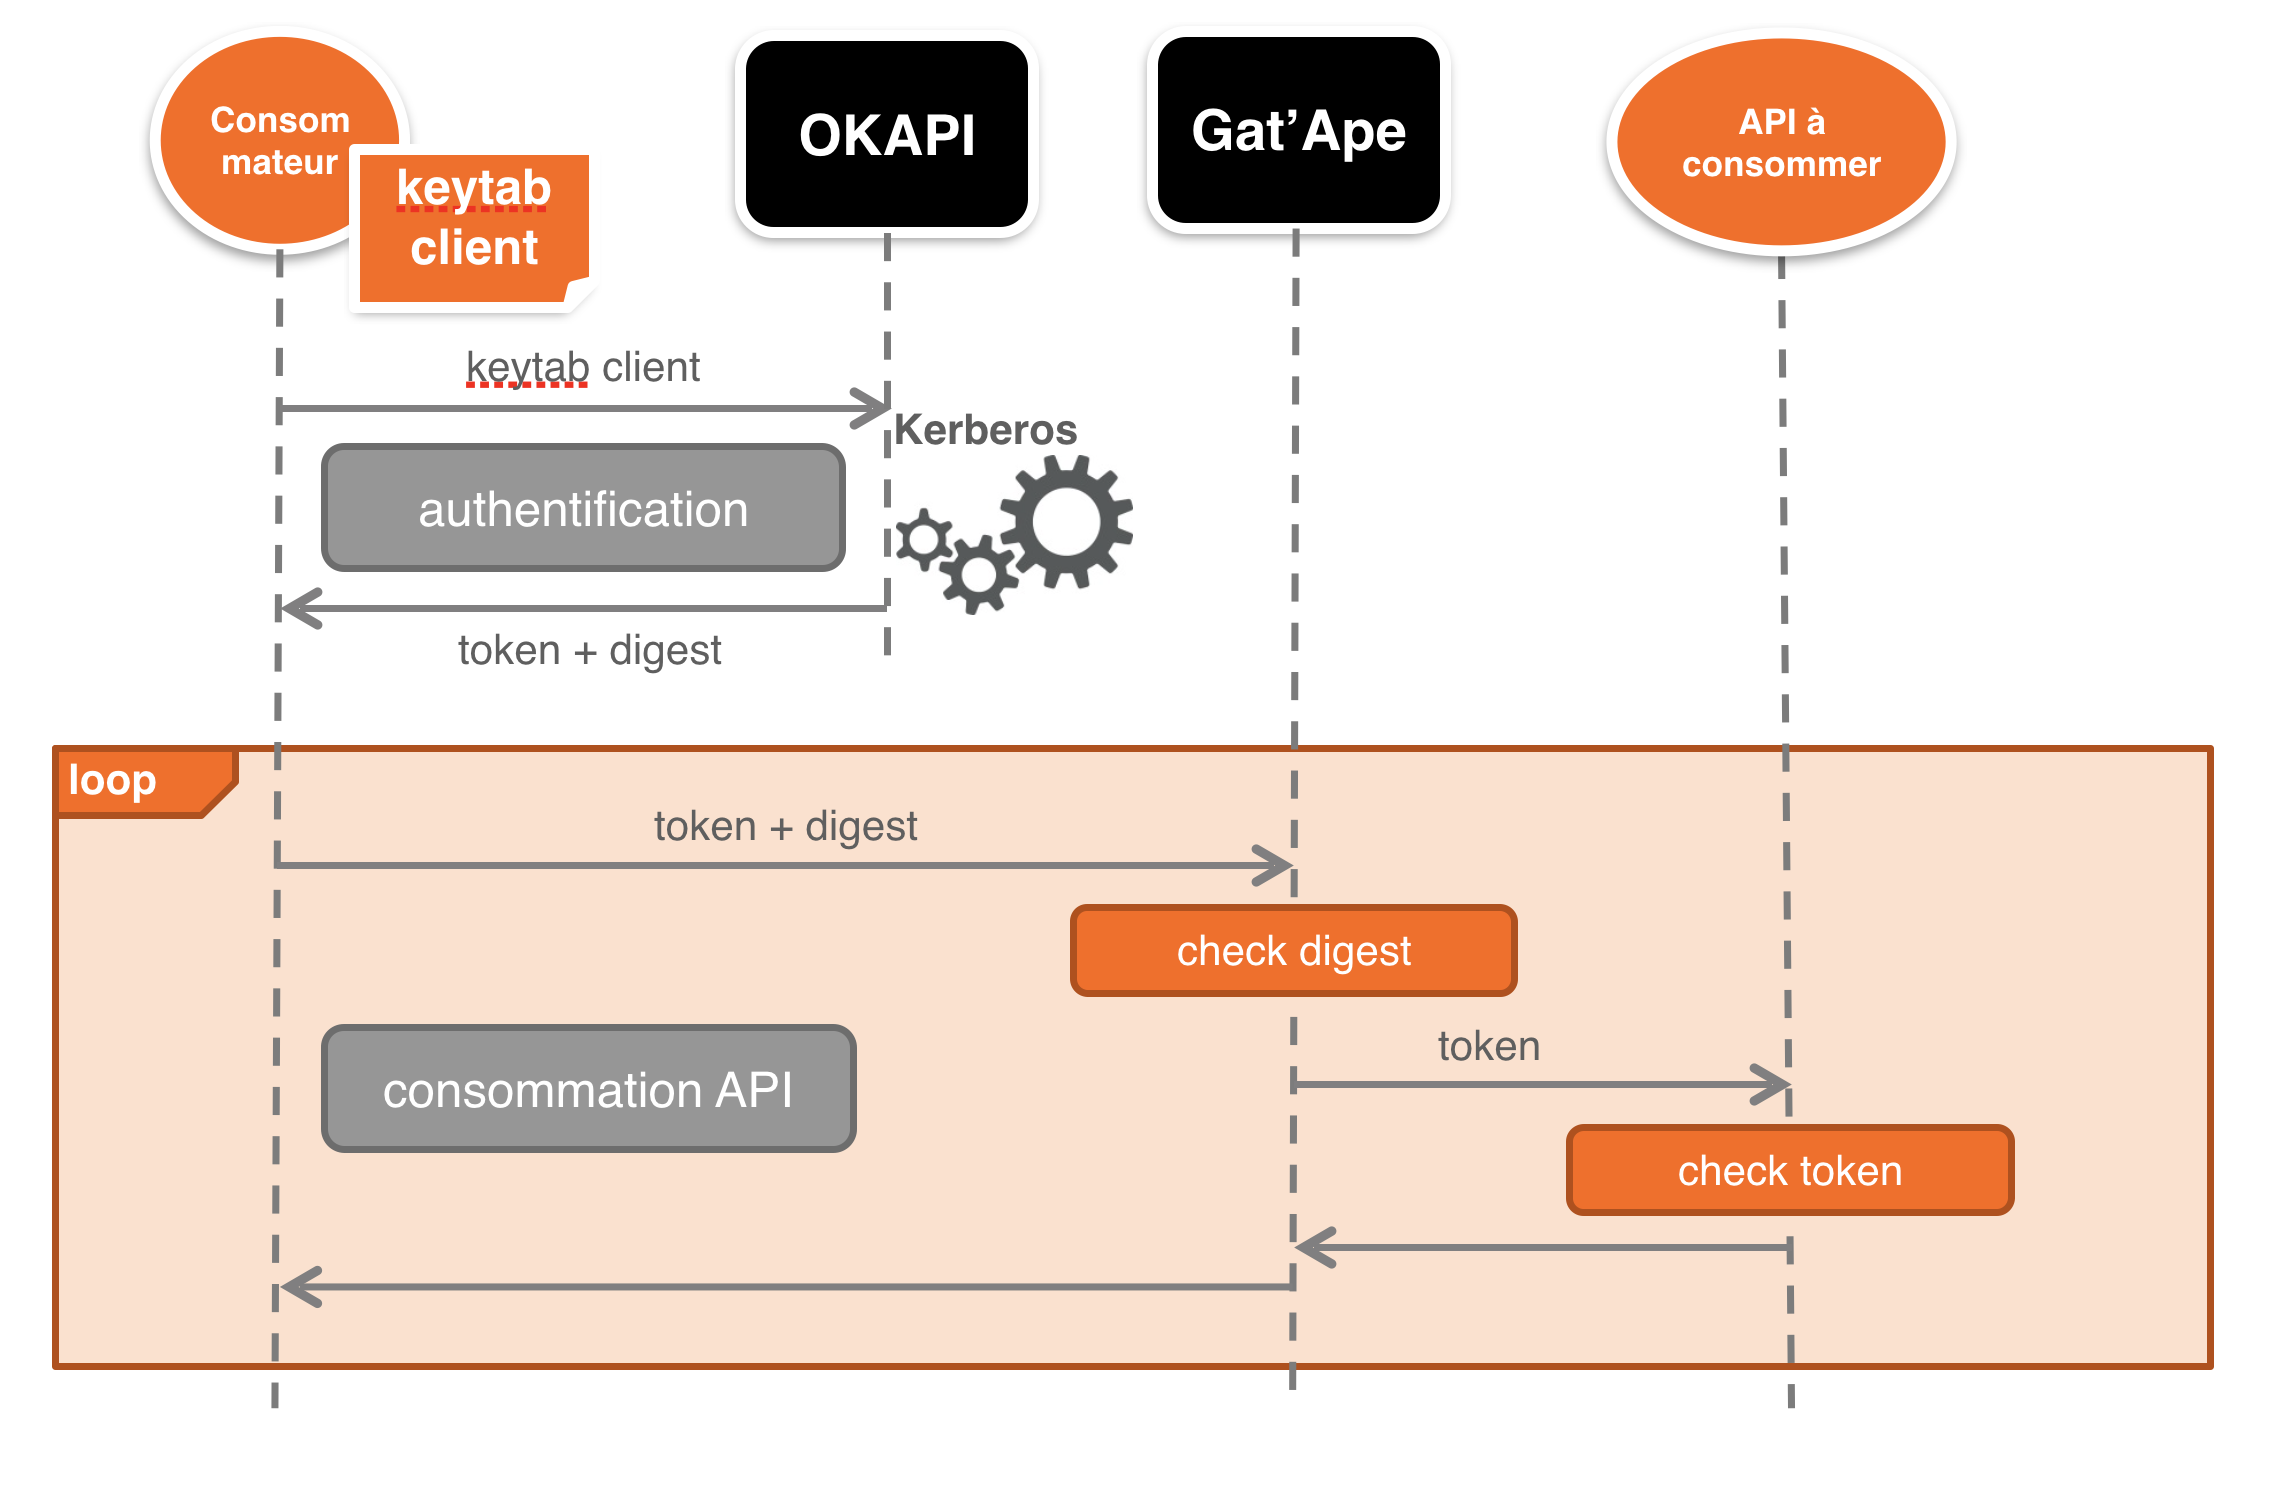
\includegraphics[width=15cm]{images/gao/gao1}
  \caption{Fonctionnement de Gat'Ape/Okapi.}
  \label{gatape}
\end{figure}



\subsection{Production}
Avant de commencer la production à proprement parlé j'ai tout d'abord du lire la documentation relative à cette API pour en comprendre l'utilité et le fonctionnement. Une fois que la fonction et le fonctionnement de cette API m'était plus clair, j'ai pris rendez vous avec le responsable solution de cette API. Nous avons fait une réunion dans laquelle je lui ai demandé les points qu'il voulait mettre en avant grâce à la vidéo et les principales innovations qu'apportait Gat'ape/okapi par rapport à l'ancienne solution. Une fois d'accord sur les points à aborder je me suis mis à produire un script, et un storyboard qui sont respectivement le texte de la vidéo et les images et animations clefs de celle ci. Une fois le script et le storyboard finalisé, j'ai de nouveau rencontré le responsable de Gat'ape/Okapi pour les lui proposer. Une fois ces documents validés, j'ai pu me lancer dans la production à proprement parler. J'ai choisi de créer un thème sobre et direct pour que les spectateurs ne se perdent pas dans les détails. Un fond blanc et les illustrations trouvées sur le site de la marque. De cette manière j'étais sûr de respecter les conditions de la charte graphique, à savoir, au mois 20\% de couleur orange sur les illustrations ainsi que les couleurs et la police officielle.\\

Au lancement de la vidéo, les logos de Gat'ape et Okapi arrivent depuis chaque côté de l'écran, présentant ainsi les deux APIs. La partie suivante de la vidéo explique brièvement la fonction générale de Gat'ape/Okapi. Les APIs exposés au travers de Gat'ape apparaissent en premier, pour symboliser le fait qu'elles sont déjà présentes et visibles, puis les consommateurs font leur apparition et ces derniers sont reliés aux APIs via des flèches en passant par le duo Gat'ape/Okapi. Vient ensuite l'explication de l'identification. Le nom du protocole d'authentification, Okapi, apparaît et est décomposé pour expliquer son acronyme. Dans un premier temps le protocole Oauth2 est expliqué comme étant le moyen de mise en relation du consommateur avec Okapi,  puis Kerberos est succinctement expliqué comme étant un protocole d'identification à base de clé secrète et de jeton. Kerberos étant crucial et complexe, j'ai choisi de l'expliciter dans la partie suivante de la vidéo autour d'une situation connue de tous, l'accès à une salle de cinéma. Dans un premier temps le spectateur, dans le cas concret : le consommateur, va récupérer au guichet (Okapi) son ticket. Une fois ceci fait, le spectateur doit passer devant l'ouvreur au point d'accès de la salle qui va déchirer le ticket et en garder une partie. Lors du contrôle (l'accès à Gat'ape), il est vérifié que les deux morceaux de tickets vont bien ensemble, si c'est le cas le spectateur peut accéder à sa séance (Le consommateur peut accéder à l'API). Il est ensuite précisé que le ticket à une durée bien définie, une séance dans le cas d'un ticket de cinéma, un Time To Live (durée de vie) paramétrable dans le cas de Gat'ape/Okapi. Il est ensuite mis en avant les possibilités qu'offre Gat'ape dans la mise en relation entre le consommateur et l'API, tels le contrôle d'accès, qui va permettre d'autoriser ou non l'accès à une API à certains consommateurs et le contrôle de trafic qui va permettre de réguler les flux d'accès en fonction de la demande des consommateurs et de la disponibilité de l'api. Pour représenter le contrôle d'accès j'ai choisi d'utiliser des croix rouges et des coches vertes afin de rester simple et compréhensible. J'ai choisi d'illustre le contrôle de trafic avec des feux tricolore que l'on voit changer de couleur pour symboliser le fait que ce contrôle n'est pas figé et se déroule en continu. La fonctionnalité mise en avant ensuite est la détection d'erreurs et d'anomalies qui est fournie par une autre API intégrée à Gat'ape, représentée par un moniteur qui contient une sorte d'électrocardiogramme qui grandit dangereusement à un moment, cette anomalie est ensuite entourée en rouge avec un panneau danger, qui représente la détection. Les fonctionnalité mentionnées ensuite sont un surcoût de temps de réponse quasi nul, qui n'impacte pas les performances, et une architecture tri site, qui assure  une très haute disponibilité. En effet, si l'un des trois site venait à subir une maintenance, une attaque ou être indisponible pour une autre raison, il y a deux autres sites qui pourront fournir l'authentification et garantir la sécurité aux consommateurs. J'ai ensuite choisi de faire un résumé des principales informations car la vidéo était un peu longue et assez détaillée sur certains points, et les personnes les moins techniques pourraient avoir décroché. Il est donc rappelé que Gat'ape permet à des APIs d'être exposées à des consommateurs qui pourront s'y connecter de manière sécurisée efficace, via l'apparition de deux logos rappelant ces informations. Il est ensuite indiqué via les logos respectifs qu'il existe un SDK pour permettre l'intégration facile de Gat'ape/Okapi à son application et qu'il existe un modèle d'API contenant Gat'ape/okapi prêt à l'usage pour les personnes souhaitant développer une API. Dans la dernière séquence, sont indiqués les liens vers la documentation et le mail de l'équipe en charge pour les personnes souhaitant avoir plus d'informations à ce sijet. 



\section{Vidéo sur Zbus}

\subsection{Contexte}

\subsection{Production}



\section{Vidép sur Valkey}

\subsection{Contexte}

\subsection{Production}

%%% Local Variables: 
%%% mode: latex
%%% TeX-master: "isae-report-template"
%%% End: 

%%% 